% Source - https://stackoverflow.com/a/73951765
% Posted by Celdor
% Retrieved 2026-03-24, License - CC BY-SA 4.0

\pgfplotsset{width=12cm,compat=1.18}
\begin{figure}[H]
    \centering
    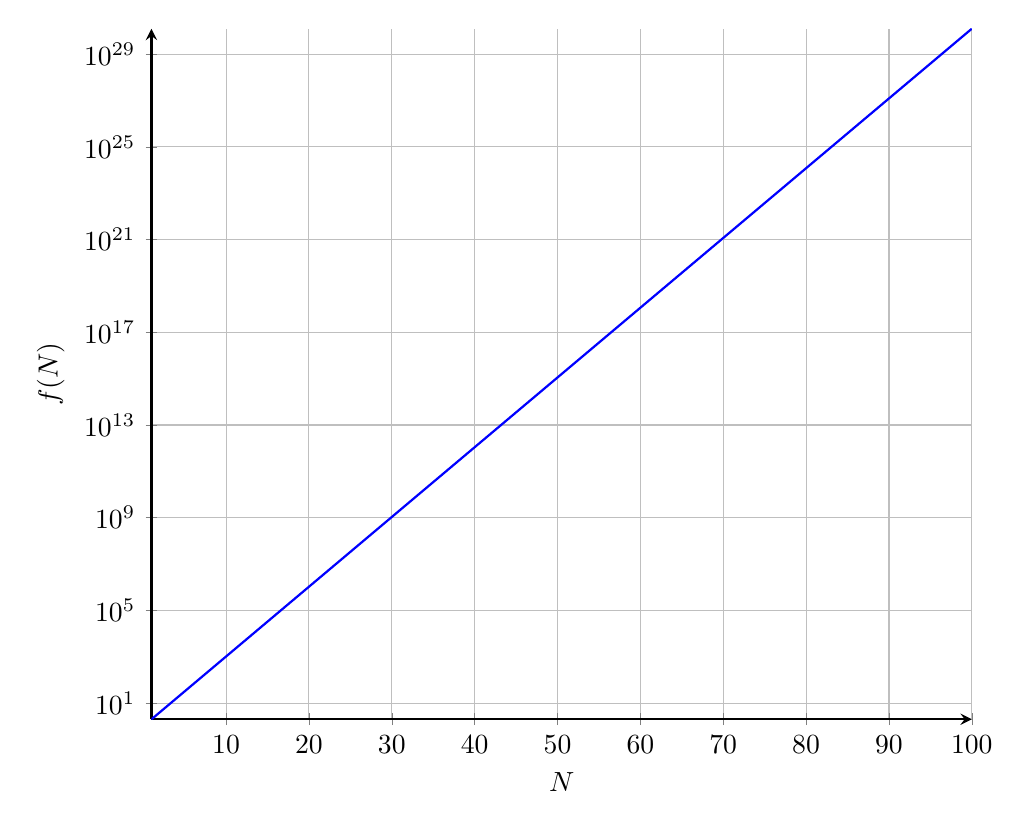
\begin{tikzpicture}
    \begin{axis}[
      axis lines=left,
      xmin=1, xmax=100,
      ymode=log,
      domain=0:100,
      samples=100,
      no markers,
      thick,
      grid=both,
      xlabel={$N$},
      ylabel={$f(N)$},
    ]
      \addplot+ {pow(2,x)};
    \end{axis}
    \end{tikzpicture}
    \caption{Prikaz $f(N)=2^N$ v logaritemski skali.}
    \label{fig:time_complexity_plot}
\end{figure}